\documentclass[a4paper,12pt]{article}
\usepackage[utf8]{inputenc}
\usepackage[margin=0.6in]{geometry}
\usepackage{amsmath, amssymb, dsfont}
\usepackage[font=footnotesize]{caption}
\usepackage{braket}
\usepackage{hyperref}
\usepackage{xcolor}
\usepackage{subfigure}
\usepackage{graphicx}
\hypersetup{
    colorlinks,
    linkcolor={blue!70!black},
    citecolor={blue!70!black},
    urlcolor={blue!70!black}
}

\newcommand\todo[1]{\textcolor{red}{#1}}

%opening
\title{A primer on quantum RAM}
\author{Olivia Di Matteo}

\begin{document}

\maketitle

\abstract{\textcolor{red}{\textbf{This document is a work in progress} and is being continuously edited.}}
\setcounter{tocdepth}{4}
\setcounter{secnumdepth}{4}
\tableofcontents

\section{Introduction and FAQ}

Quantum RAM (qRAM) has gained some notoriety in the past few years, and attitudes toward it depend quite heavily on the circles you run in. 
The goal of this set of notes is to provide a general overview of the subject, as well as discuss some very specific implementations. 
It is meant to be a companion to the Q\# qRAM libraries we are writing (cite the repo), but can also serve as a standalone reference.


In my experience, explaining qRAM to someone boils down to answering a handful of key questions. 
I'll provide some potentially unsatisfactory answers up front, but go into far more detail in the next few sections\footnote{Those details may not be satisfactory either.}.

\begin{enumerate} 
 \item \textbf{Do I need a qRAM?}
  \emph{Sometimes}. You'll need a qRAM, or some more general means of \emph{quantum state preparation} in quantum machine learning (QML) algorithms that require you to load in classical data, or query an oracle that returns classical data. 
  I've heard a number of stories of people working on QML being actively discouraged from doing so because ``QML won't work without a qRAM''. 
  That's just not true, because \emph{many QML algorithms do not need a qRAM}.
  Now, whether or not they yield any quantum advantage is a separate question, and won't be discussed here. 
  The key point I want to make is that \emph{some} QML algorithms need a qRAM, and they will potentially run into trouble as per the next question.
 \item \textbf{Can we design an efficient qRAM?} \emph{Maybe.} 
 In this primer we'll take a look at proposals that will in principle run in polynomial depth, and others that scale far worse. 
 There are some very interesting qubit-time tradeoffs one can explore, in particular if the data being stored has some sort of underlying structure. 
 Regardless, even if we can design an efficient circuit, we'd also like something that is efficient in a fault-tolerant setting, and this is potentially very expensive.
 \item \textbf{Can I build one?} \emph{Maybe.} No one has actually done so, but there are a handful of hardware proposals that will be discussed in more detail in \autoref{sec:hardware}. 
\end{enumerate}


%%%%%%%%%%%%%%%%%%%%%%%%%%%%%%%%%%%%%%%%%%%%%%%%%%%%%%%%%%%%%%%%%%%%%%%%%%%%%%%%%%
%%%%%%%%%%%%%%%%%%%%%%%%%%%%%%%%%%%%%%%%%%%%%%%%%%%%%%%%%%%%%%%%%%%%%%%%%%%%%%%%%%
%%%%%%%%%%%%%%%%%%%%%%%%%%%%%%%%%%%%%%%%%%%%%%%%%%%%%%%%%%%%%%%%%%%%%%%%%%%%%%%%%%
%%%%%%%%%%%%%%%%%%%%%%%%%%%%%%%%%%%%%%%%%%%%%%%%%%%%%%%%%%%%%%%%%%%%%%%%%%%%%%%%%%
%%%%%%%%%%%%%%%%%%%%%%%%%%%%%%%%%%%%%%%%%%%%%%%%%%%%%%%%%%%%%%%%%%%%%%%%%%%%%%%%%%

\section{A brief history of the brief history of quantum machine learning}
\label{sec:qml}

%%%%%%%%%%%%%%%%%%%%%%%%%%%%%%%%%%%%%%%%%%%%%%%%%%%%%%%%%%%%%%%%%%%%%%%%%%%%%%%%%%
%%%%%%%%%%%%%%%%%%%%%%%%%%%%%%%%%%%%%%%%%%%%%%%%%%%%%%%%%%%%%%%%%%%%%%%%%%%%%%%%%%
%%%%%%%%%%%%%%%%%%%%%%%%%%%%%%%%%%%%%%%%%%%%%%%%%%%%%%%%%%%%%%%%%%%%%%%%%%%%%%%%%%
%%%%%%%%%%%%%%%%%%%%%%%%%%%%%%%%%%%%%%%%%%%%%%%%%%%%%%%%%%%%%%%%%%%%%%%%%%%%%%%%%%
%%%%%%%%%%%%%%%%%%%%%%%%%%%%%%%%%%%%%%%%%%%%%%%%%%%%%%%%%%%%%%%%%%%%%%%%%%%%%%%%%%

\section{Encoding classical data on a quantum computer}

\label{sec:encoding}

There is a nice overview of the encodings below in \cite{Schuld2018}.

\subsection{Basis encoding}

Give overview of the basis encoding, i.e.
\begin{equation}
 \hbox{data} \enskip 01001 \rightarrow \ket{01001}
\end{equation}


\subsection{Quantum RAM / ROM}

Query as bits in superposition:
\begin{equation}
 \sum_i \ket{i} \ket{0} \rightarrow \sum_i \ket{i} \ket{b_i}
\end{equation}

Query as phase in superposition (applications to Grover)
\begin{equation}
 \sum_i \ket{i} \rightarrow \sum_i (-1)^{b_i} \ket{i}
\end{equation}


\subsection{Quantum state preparation (amplitude encoding)}

Given some vector $\mathbf{a} = \left( a_0, \cdots,  a_{n-1} \right)$, create the quantum state
\begin{equation}
 \ket{\psi} = \sum_{i=0}^{n-1} a_i \ket{i}
\end{equation}

Discuss how this relies on having a qROM as an underlying subroutine.


%%%%%%%%%%%%%%%%%%%%%%%%%%%%%%%%%%%%%%%%%%%%%%%%%%%%%%%%%%%%%%%%%%%%%%%%%%%%%%%%%%
%%%%%%%%%%%%%%%%%%%%%%%%%%%%%%%%%%%%%%%%%%%%%%%%%%%%%%%%%%%%%%%%%%%%%%%%%%%%%%%%%%
%%%%%%%%%%%%%%%%%%%%%%%%%%%%%%%%%%%%%%%%%%%%%%%%%%%%%%%%%%%%%%%%%%%%%%%%%%%%%%%%%%
%%%%%%%%%%%%%%%%%%%%%%%%%%%%%%%%%%%%%%%%%%%%%%%%%%%%%%%%%%%%%%%%%%%%%%%%%%%%%%%%%%
%%%%%%%%%%%%%%%%%%%%%%%%%%%%%%%%%%%%%%%%%%%%%%%%%%%%%%%%%%%%%%%%%%%%%%%%%%%%%%%%%%


\section{Bucket-brigade quantum RAM}
\label{sec:bb}

Architectures for qRAM began to emerge roughly a decade ago with the bucket brigade RAM model of \cite{Giovannetti2008, Giovannetti2008b}. 
The particular storage model of RAM that is used is a binary tree, where $2^n$ bits are located at the leaves of an $n$-level binary tree, as depicted in \autoref{fig:fanout-ram-sequence}. 
We will first take a graphical look at the bucket brigade algorithm; following this, we will see it modelled as a quantum circuit.

\subsection{Increasing efficiency of RAM with a bucket brigade}

The motiviation for bucket brigade lies in a less efficient type of RAM denoted as `fanout RAM'. 
In the fanout RAM, the nodes of this tree are transistors that, depending on their state, will route incoming current left or right towards the next level of the tree. 
Each level of the tree is associated to an address bit; the value of the address bit can set a level-specific switch that tells all transistors in the level to send current left, or send current right. 
This is shown in the right panel of \autoref{fig:fanout-ram-sequence}, and has the effect creating only one complete path from the root of the tree to a leaf.


The issue with fanout RAM in this form is its efficiency - for an $n$-bit address, we are turning on $2^n - 1$ transistors, while only $n$ of them are involved in the actual query. 
A further issue arises if we make a direct translation into qubits. 
Suppose we replace each node of the tree with a qubit; we can let its $\ket{0}$ state indicate `route left', and its $\ket{1}$ state indicate `route right'. 
When we go to initialize the qubits to create the path, the $k$'th address qubit will have to couple with $2^k$ node qubits. 
This is a very precarious superposition, especially in an era where coherence times are low and multi-qubit operations are significantly noisier than single-qubit ones.

\begin{figure}[ht!]
 \centering
  \captionsetup{width=.89\linewidth}
 \begin{subfigure}
    \centering
    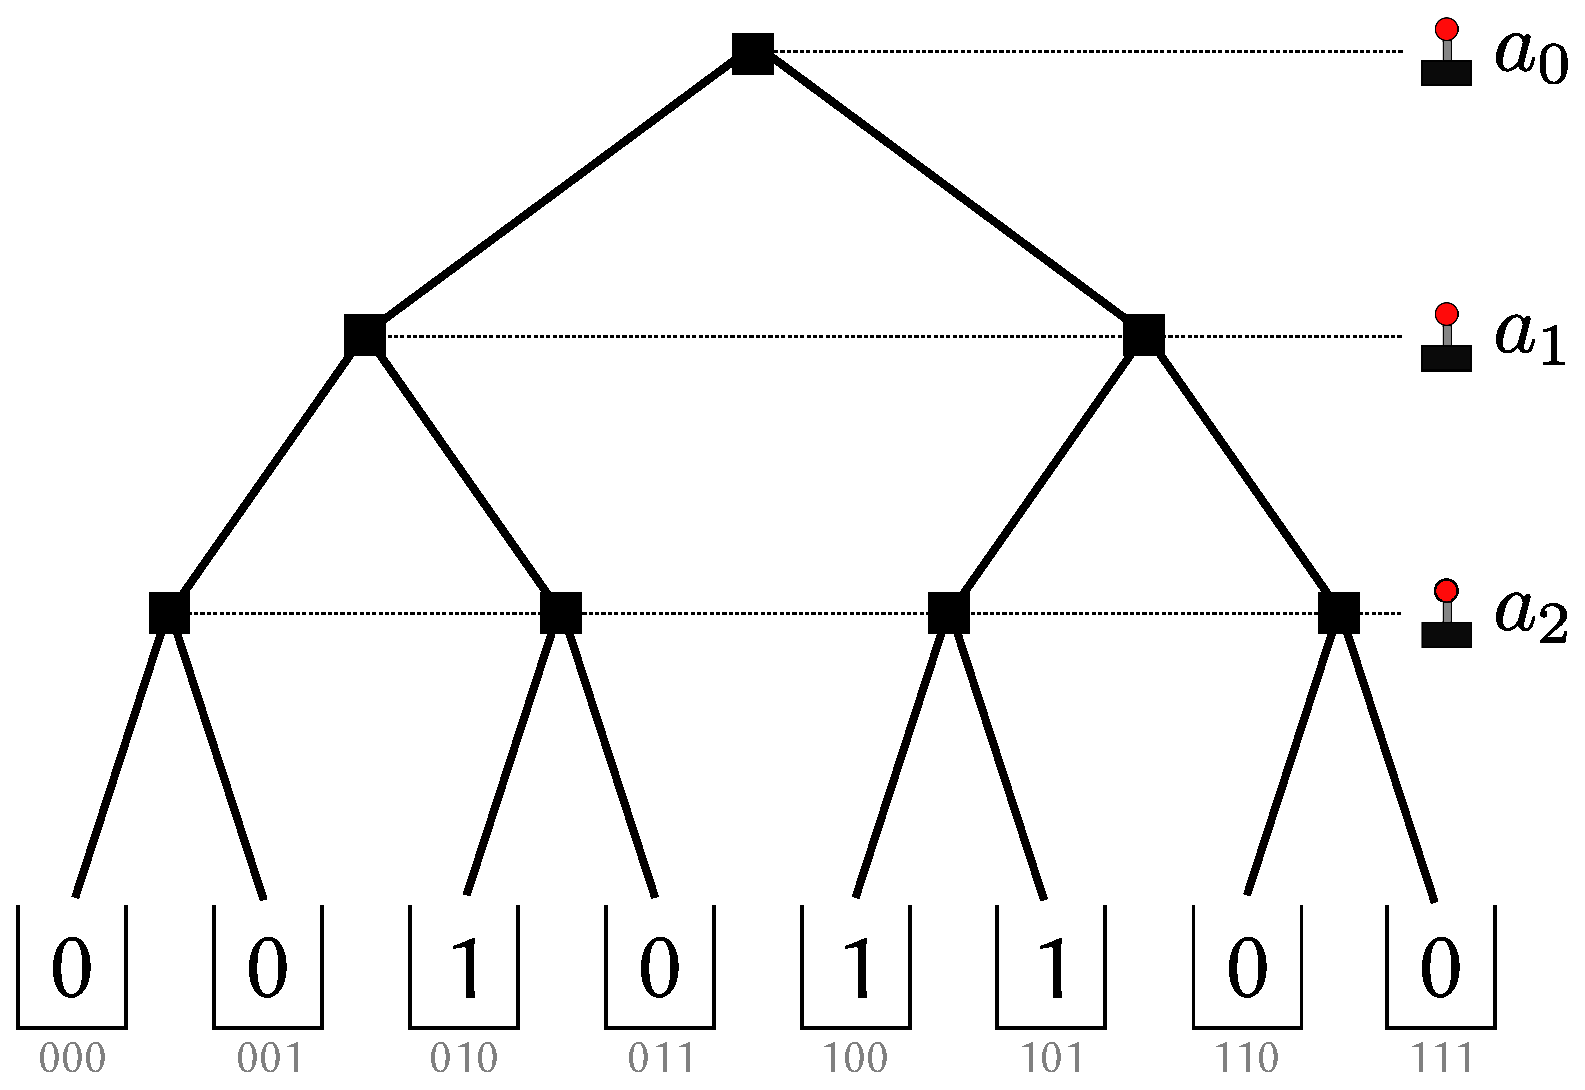
\includegraphics[height=2in]{images/fanout-ram}
 \end{subfigure}
  \hspace{0.5cm}
  \begin{subfigure}
    \centering
    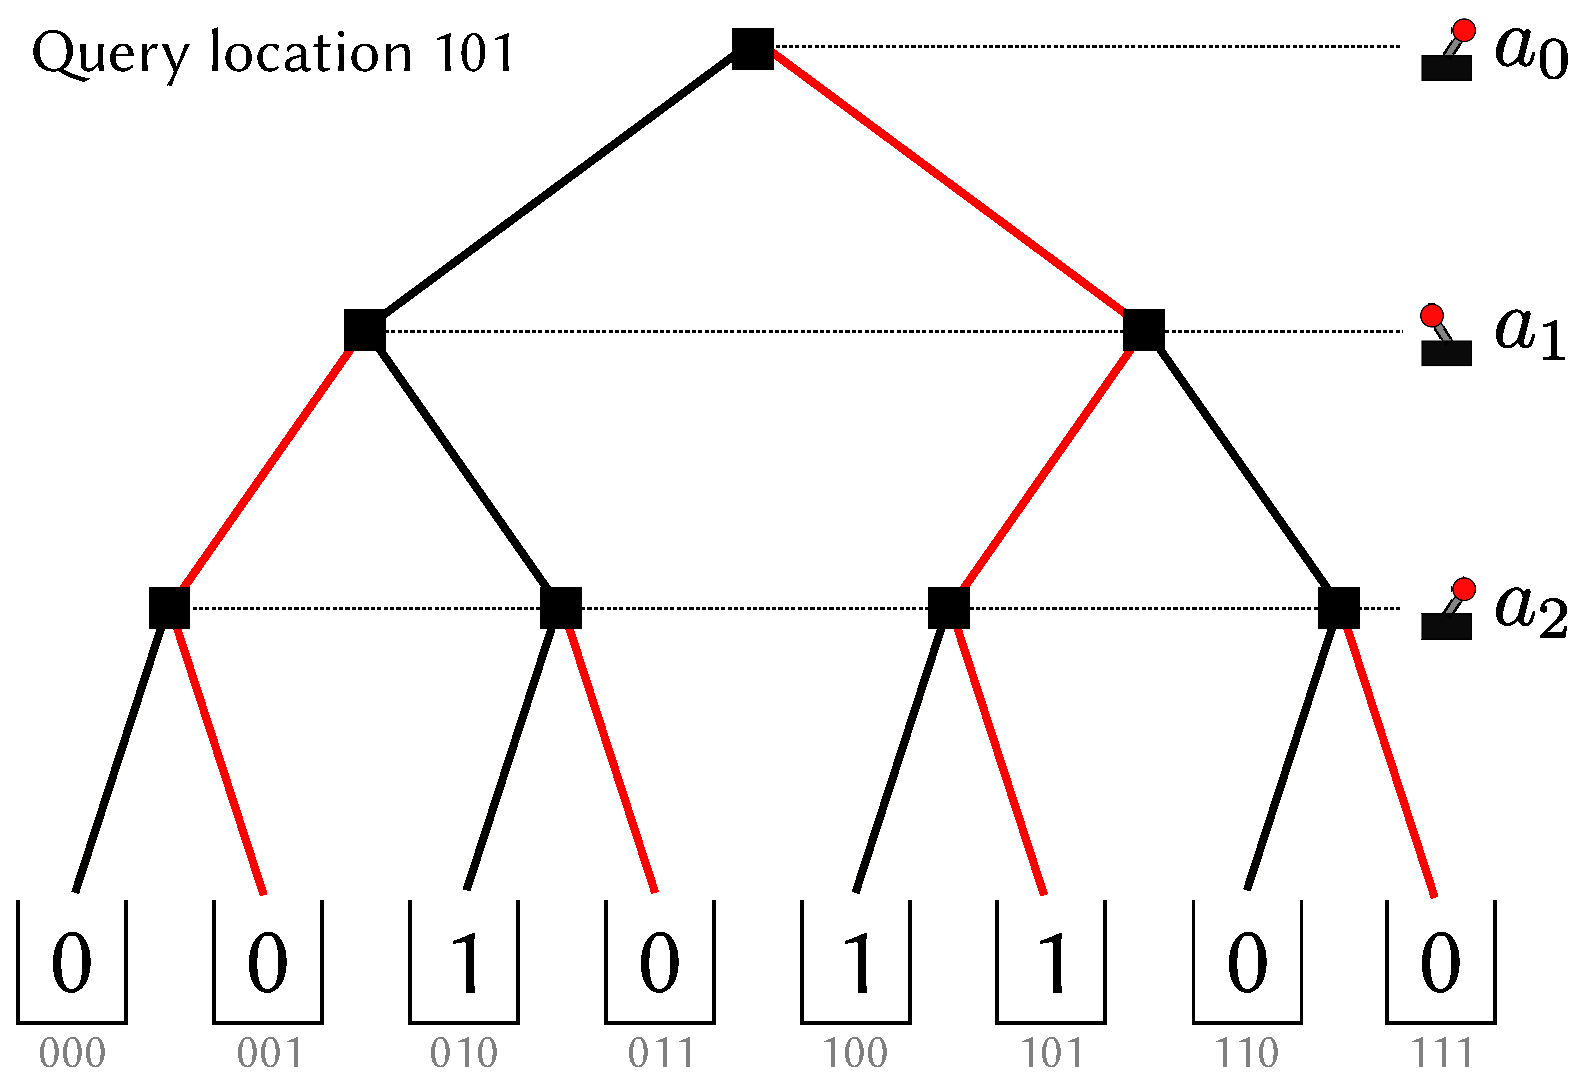
\includegraphics[height=2in]{images/fanout-ram-queried}
 \end{subfigure} 
    \caption{(Left) Schematic of a `fan-out RAM', whose inefficiencies were the motivation for the bucket brigade RAM. 
    For an $n$-bit address, an $n$-level binary tree stores the memory contents at its leaves. 
    At each node of the tree is a transistor that can direct current right, or left. 
    Within each level of the tree, all transistors are controlled by a switch that can either direct them all to route current left, or all right. 
    (Right) To query the memory contents, the directions of the switches are set according to the address bits (one bit per level of the tree). 
    This creates a single path from the root node to the desired cell.}
    \label{fig:fanout-ram-sequence}
\end{figure}

The bucket-brigade model is an improvement that addresses both of these issues.
Rather than using qubits at each node, we use \emph{qutrits}, or three-state systems. 
In what follows we will discuss the quantum case, but the methodology is the same for the classical case (it uses trits instead of bits).

In the top left of \autoref{fig:bb-sequence} is our familiar binary tree. 
At each node sits a qutrit whose states are descriptively named $\ket{\hbox{wait}}, \ket{\hbox{left}}, \ket{\hbox{right}}$. 
All the qutrits begin in $\ket{\hbox{wait}}$. 
To perform a query, \emph{address qubits} are introduced to the tree one by one; the $k$'th address qubit will effect an operation in the $k$'th level of the tree to carve a path to the desired memory cell.

The key to the bucket brigade model is to define a unitary transformation that allows address qubits to alter the state of the qutrit nodes depending on their own state. 
Specifically, we need to find some unitary that performs:
\begin{eqnarray}
 U(\ket{0}\ket{\hbox{wait}}) &\rightarrow& \ket{s}\ket{\hbox{left}} \\
 U(\ket{1}\ket{\hbox{wait}}) &\rightarrow& \ket{s}\ket{\hbox{right}}
\end{eqnarray}
Here, $\ket{s}$ refers to some arbitrary state; we don't particularly care what it is, as $U$ is reversible and will be undone later on.

When an address qubit reaches a qutrit in the $\ket{\hbox{wait}}$, $U$ is performed. 
If it instead encounters $\ket{\hbox{left}}$ or $\ket{\hbox{right}}$ it `passes through' the node without altering it, and continues traveling along the path until it reaches its particular level. 
This is shown in the top right of \autoref{fig:bb-sequence}.

The bottom half of \autoref{fig:bb-sequence} describes how the contents of the memory are retrieved. 
After all the address qubits are sent, a `quantum bus' qubit traverses the path, couples to the desired memory cell to gather the data, and is reflected back the way it came. 
As it passes upwards through the tree, it re-initializes the qutrits back to $\ket{\hbox{wait}}$ by running $U^\dag$. 
Note that such an algorithm allows us to query in superposition, as all operations are unitary.


\begin{figure}
 \centering  
 \captionsetup{width=.89\linewidth}
 \begin{subfigure}
    \centering
    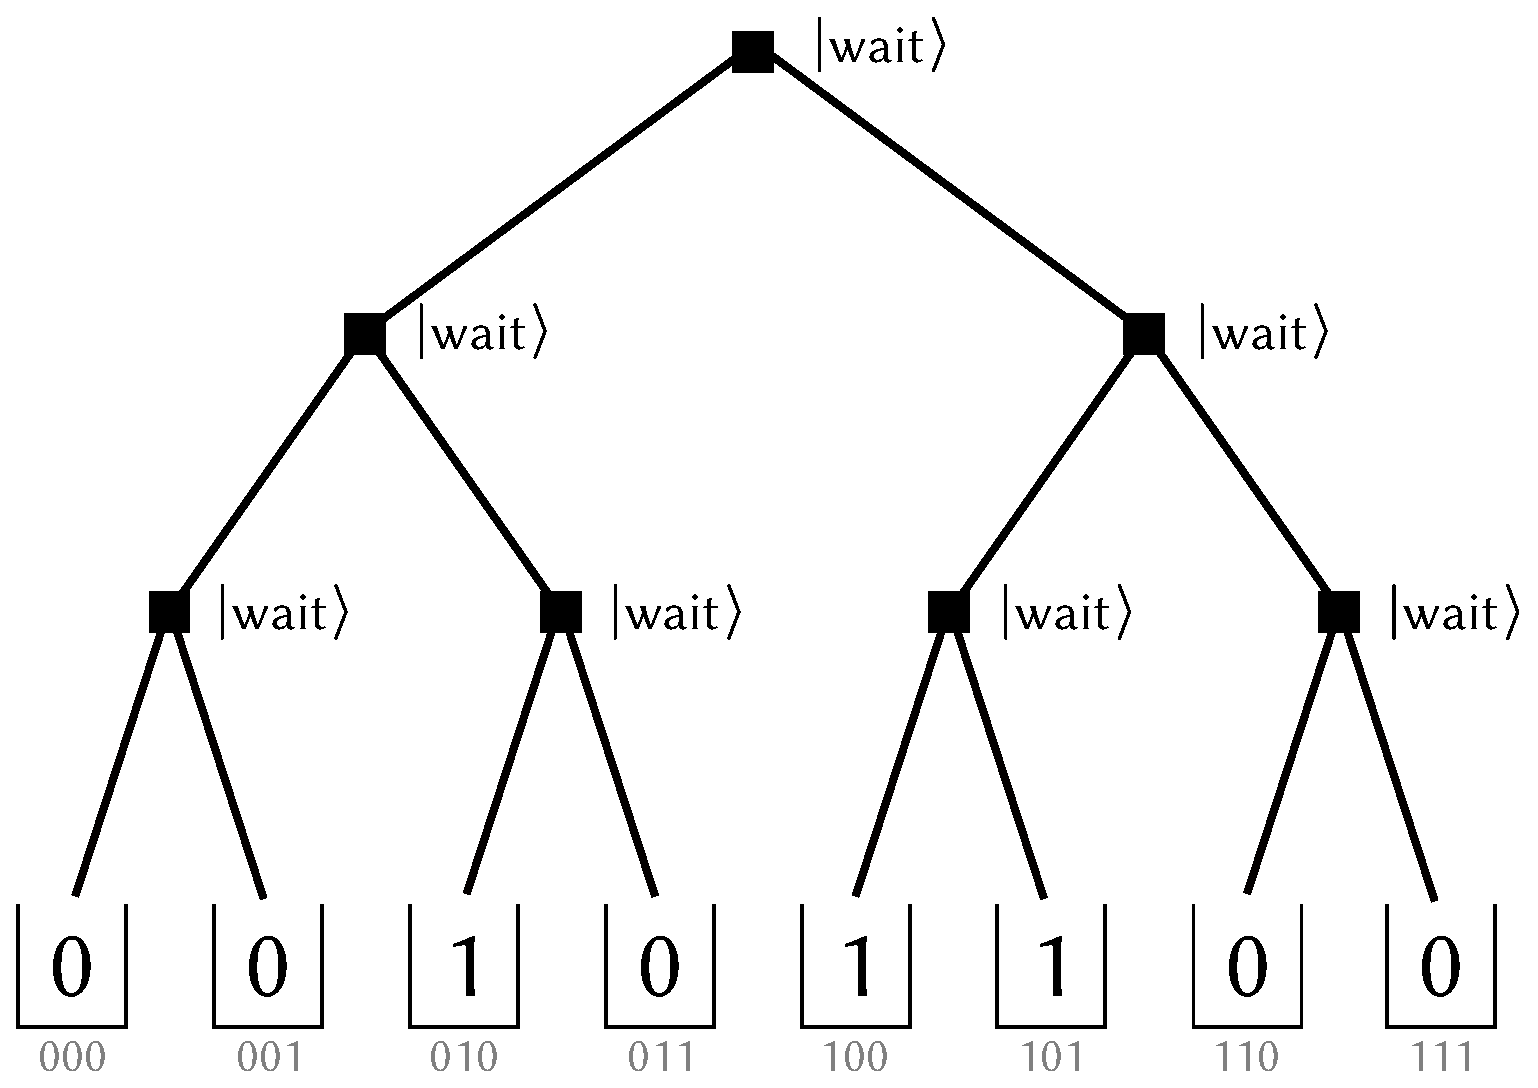
\includegraphics[height=2in]{images/bb-00}
 \end{subfigure}
  \hspace{0.5cm}
  \begin{subfigure}
    \centering
    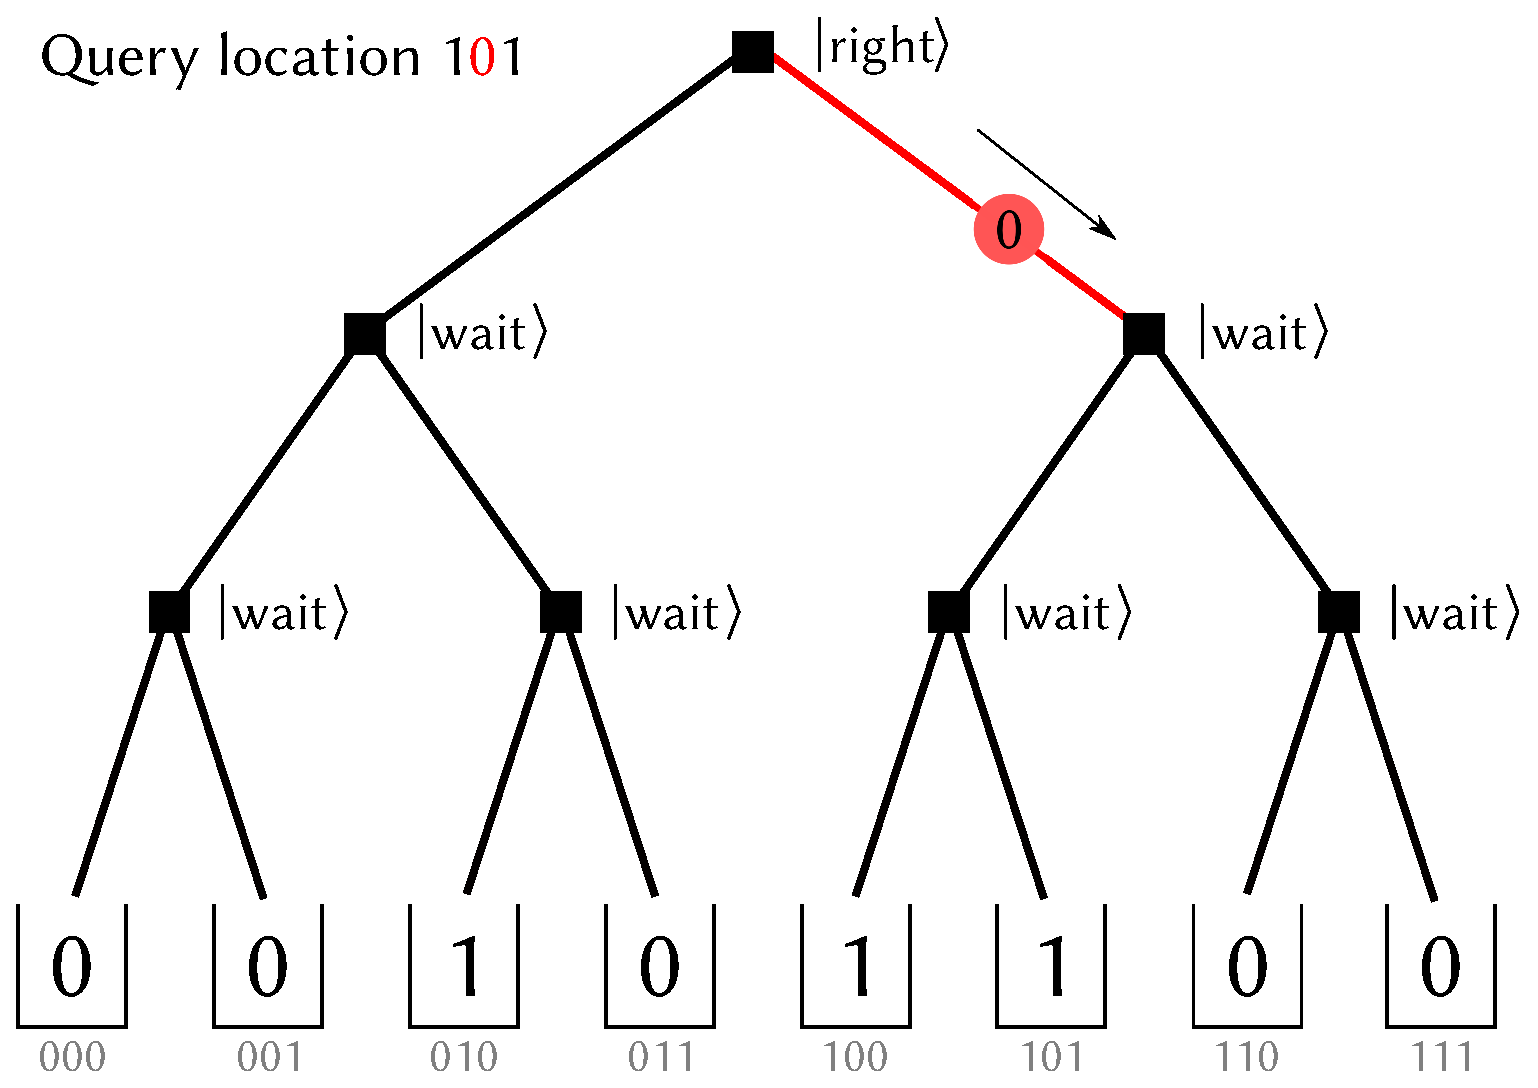
\includegraphics[height=2in]{images/bb-01}
 \end{subfigure} \\
    \vspace{0.5cm}
     \begin{subfigure}
        \centering
        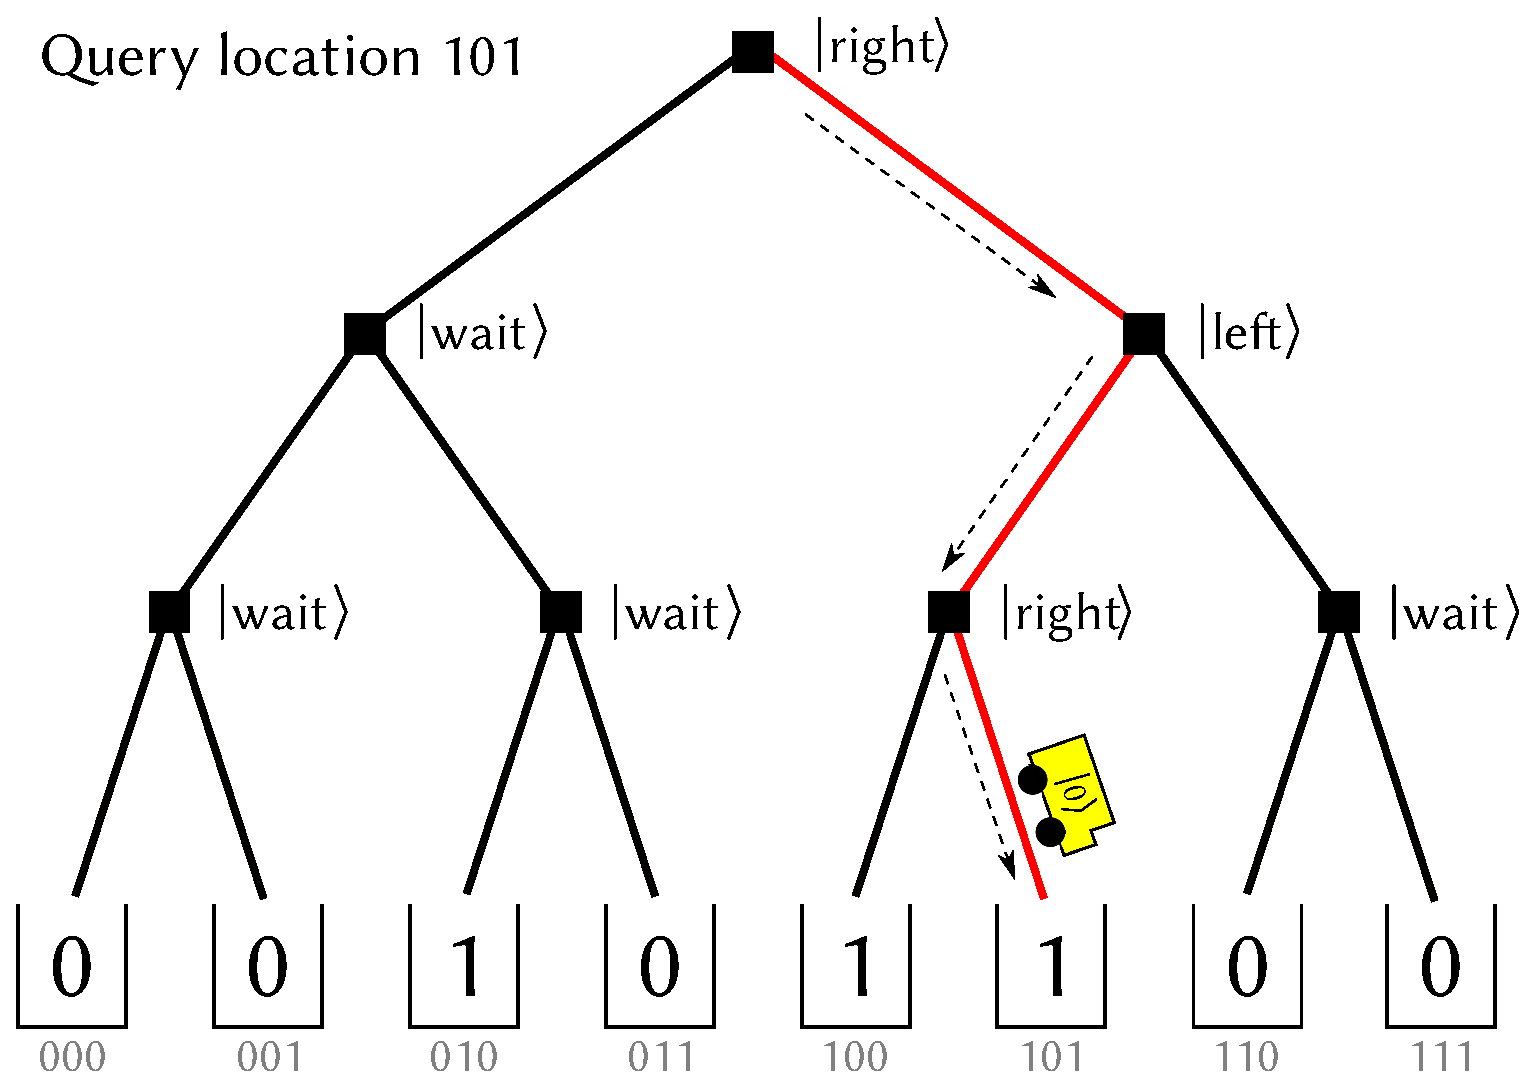
\includegraphics[height=2in]{images/bb-02}
    \end{subfigure}
    \hspace{0.5cm}
    \begin{subfigure}
        \centering
        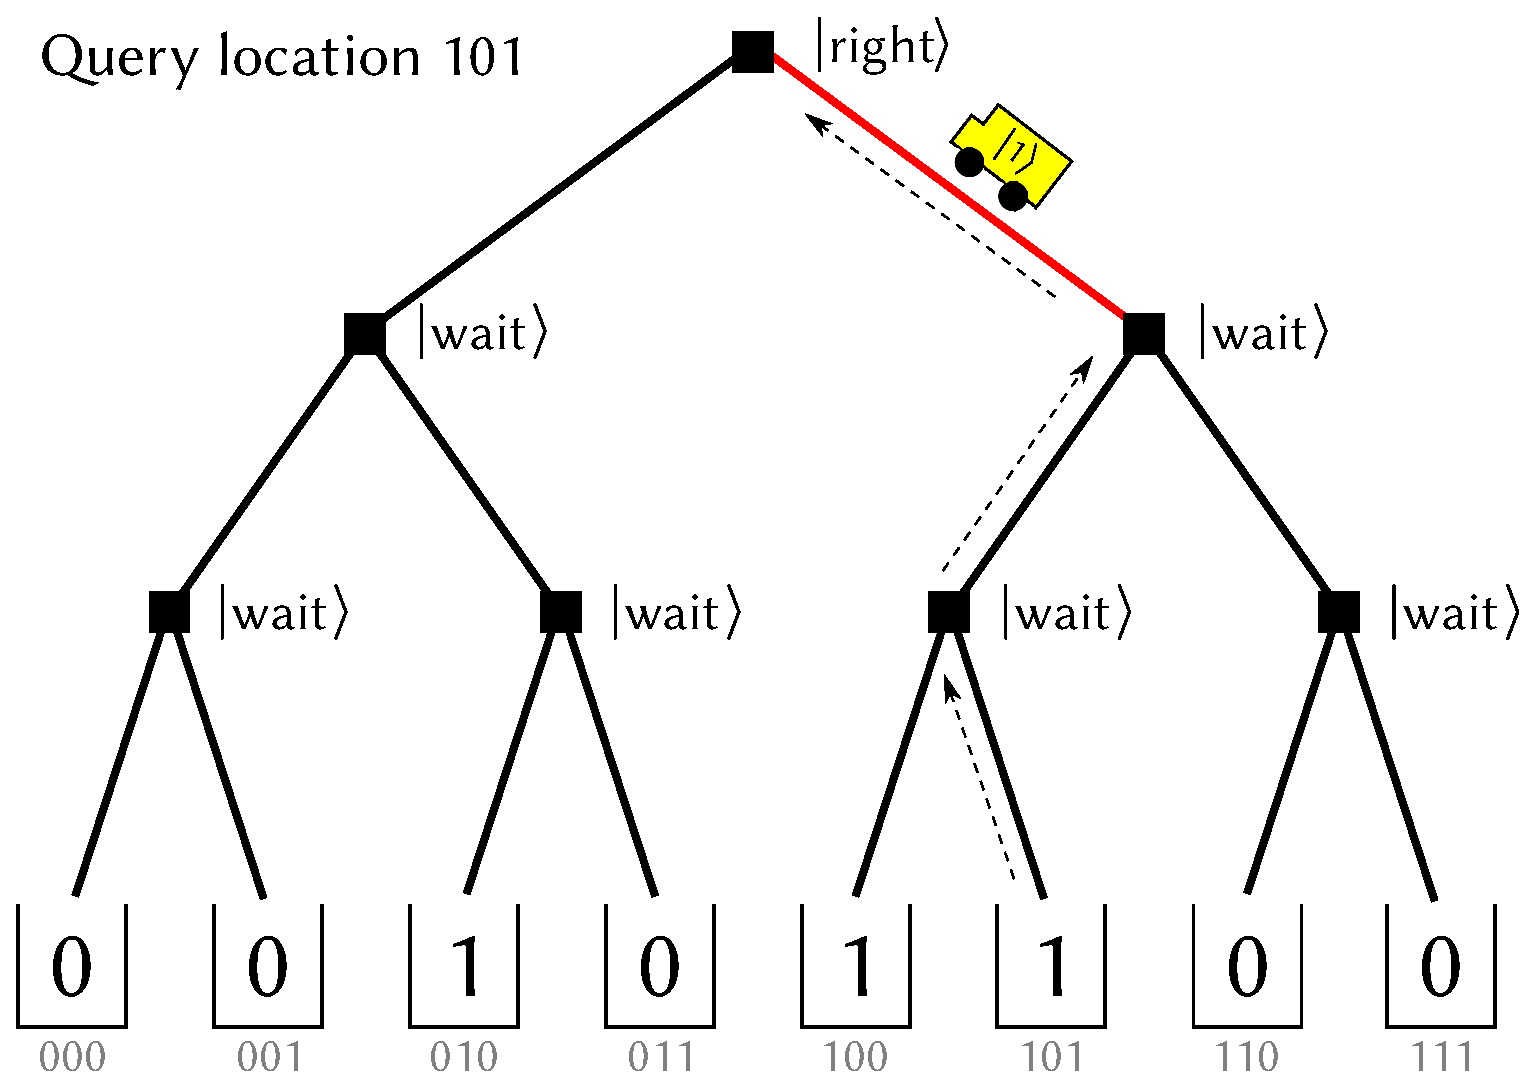
\includegraphics[height=2in]{images/bb-03}
    \end{subfigure}
    \caption{Schematic of a bucket brigade quantum RAM query. 
    (Top left) Memory contents are stored in the leaves of a binary tree, whose nodes are denoted by qutrits with possible states $\ket{\hbox{wait}}, \ket{\hbox{left}}$, and $\ket{\hbox{right}}$. 
    (Top right) A bucket brigade RAM query is set up by sequentially sending in address qubits to change the qutrit states until a path to the desired cell is created. 
    (Bottom left) To extract the contents of the memory cell, a `bus' photon is used.
    The photon is directed to the desired cell by the qutrits, where it couples to the memory cell and copies its contents. 
    (Bottom right) The bus photon travels back through the qRAM, resetting the qutrit states to $\ket{\hbox{wait}}$ on its way out.}
    \label{fig:bb-sequence}
\end{figure}



To see how efficiency is improved let's count the number of unitary operations.
The first address qubit performs one operation by coupling with the root qutrit.
The second qubit performs two, the root qutrit and then the qutrit in the second layer. The third performs three, and so on.
This means to set the qutrits takes $n(n+1)/2$ operations, more succinctly represented as $O(n^2)$. 
The bus qubit performs only $2n + 1$ operations, which does not worsen this complexity. 
As this is polynomial in the address bit size, the bucket brigade qRAM appears to be efficient. 
It is also claimed that, since only $n$ of the qutrits are involved in the query (rather than all $2^n-1$), it is potentially possible to get away with a worse error rate $O(1/n^2)$, and leave the idle qutrits uncorrected. 
\textbf{I have to go check my notes, this paragraph needs to be improved}.

\begin{enumerate} 
 \item \textbf{What happens when we query in superposition?} 
  \emph{I don't have a satisfactory answer for this.} 
  The claimed advantage comes partially from the fact that we only need to tinker with $n$ of the qutrits; but if we query in superposition, don't we still have to handle all $2^n - 1$ of them anyways?
 \item \textbf{Can we actually get away without error correction?} \emph{Potentially}. 
 It has been shown that in cases where there are a superpolynomial amount of queries to the qRAM (for example, in Grover's algorithm), the error rate of the qRAM must be superpolynomially small \cite{Regev2008}, in which case we will in fact need error correction \cite{Arunachalam2015}. 
 That said, in situations where the number of queries is small, it may be possible yet to get away without it, in which case bucket brigade provides a substantial improvement in the number of operations that must be performed.
\end{enumerate}



\subsection{Bit query circuit model}

While conceptually simple, the bucket brigade model as described in the previous section does not lend itself very well to implementation on our present day machines. 
For one, it requires both qutrits and qubits; furthermore, the operations are not specified in the usual parlance of the circuit model - how do we implement this $U$, and the routing?

A circuit model for bucket brigade qRAM was presented in \cite{Arunachalam2015}.
\autoref{fig:bb-combined} contains a re-drawn version of these circuits in order to highlight the structure of the algorithm as well as the patterns of gates that are used to perform the query.

\begin{figure}
 \centering
  \captionsetup{width=.89\linewidth}
 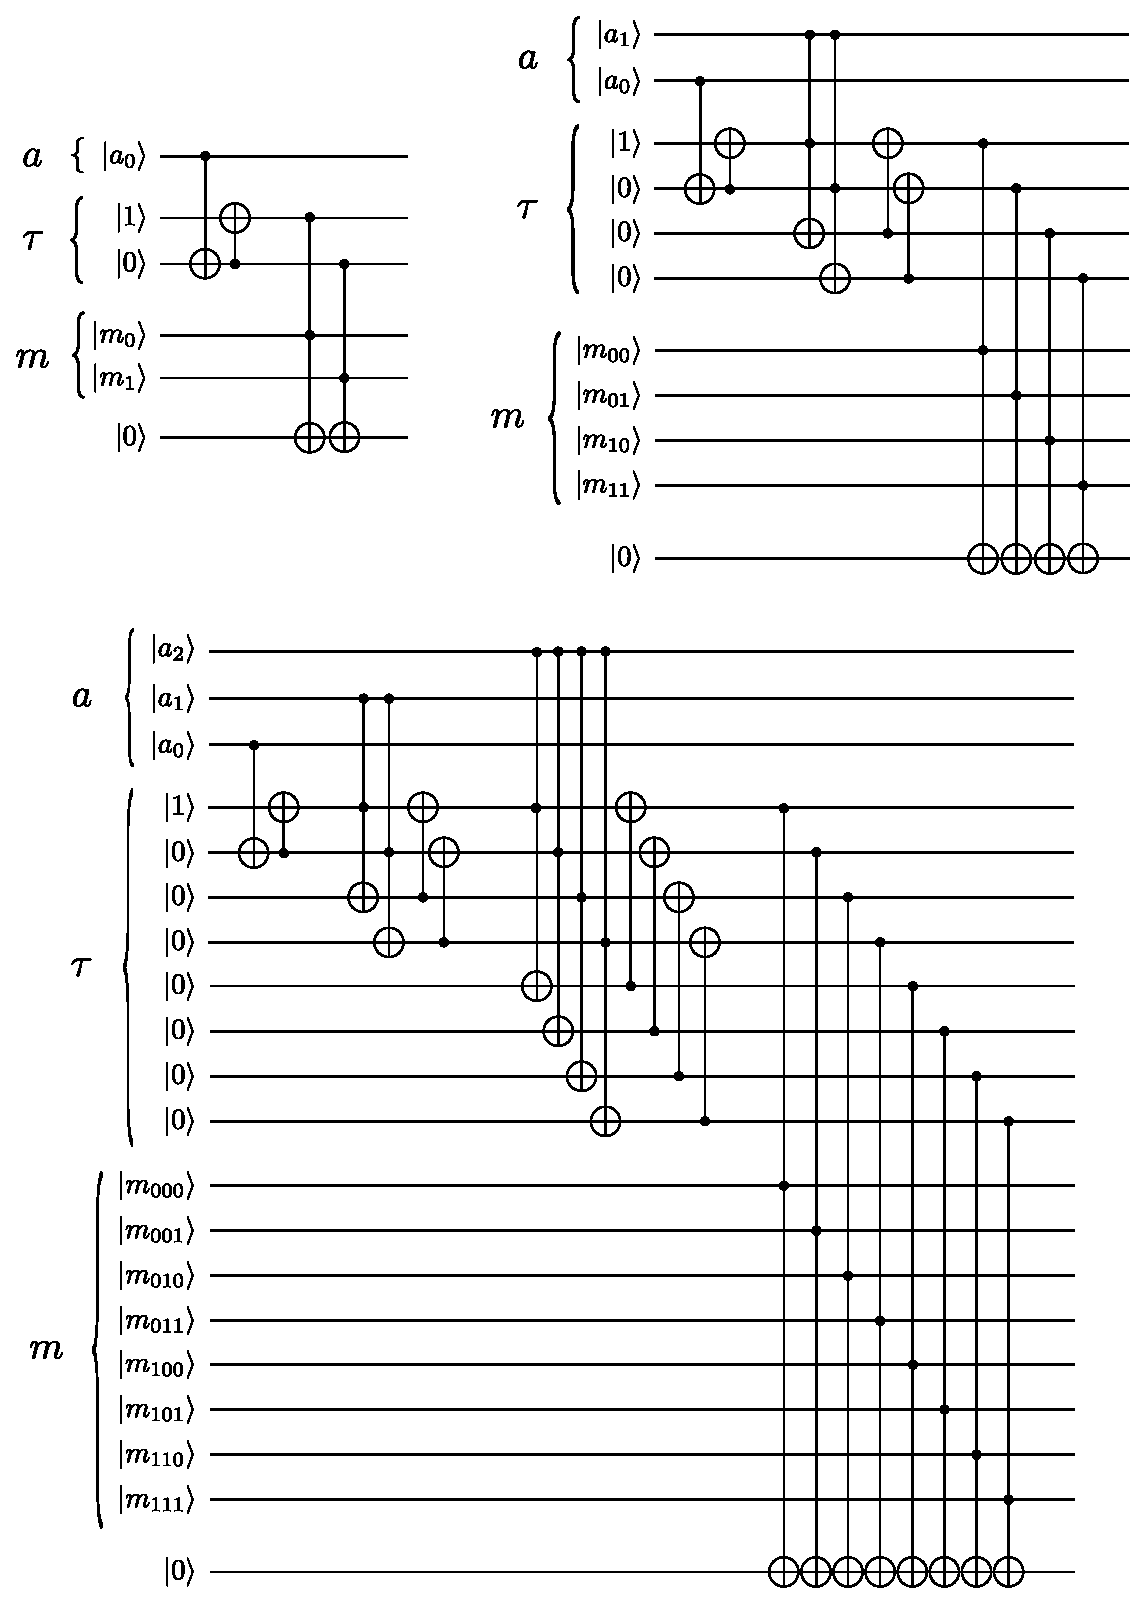
\includegraphics[scale=0.8]{images/bb-combined}
 \caption{\textbf{For pedagogical purposes; not most optimal}. 
 (Top left) A bucket brigade circuit for a 1-qubit address (2 memory cells). 
 (Top right) A bucket brigade circuit for a 2-qubit address. 
 The first 6 gates are a fanout of the address bits to the auxiliary `trigger' register, denoted by $\tau$. 
 A cascade of Toffolis then couples the memory cells to the output. 
 To make the query fully reversible, the fanout component must be repeated. 
 The subscripts on the memory cells are ordered from top to bottom of the address register, i.e. $a_{n-1}, a_{n-2}, \ldots, a_0$. 
 (Bottom) A bucket brigade circuit for a 3-qubit address, highlighting the pattern that emerges in the construction of this circuit. 
 The fanout component is recursive, with the 1- and 2-qubit fanout portions appearing.}
 \label{fig:bb-combined}
\end{figure}


The bucket brigade circuit model consists of four registers of qubits. 
To query an $n$-bit address, we require:
\begin{itemize}
 \item An address register, $a$, of $n$ qubits
 \item A memory register $m$ with $2^n$ qubits containing the stored values (i.e. qubits in $\ket{0}$ or $\ket{1}$.
 \item An auxiliary register $\tau$ with $2^n$ qubits to trigger readout of the memory register
 \item An output register
\end{itemize}

To perform a query, the address register is first `fanned out' onto the auxiliary register $\tau$ in such a way that it produces a `one-hot' encoding of the addresses to be queried. 
For example, if we want to query at address $\ket{i}$, the fanout will set the $i$'th qubit of $\tau$ to $\ket{1}$. 
This then couples to the $i$'th qubit of the memory register using a Toffoli, and changes the output bit depending on the contents. 
Finally, note that for full reversibility, the fanout must be run in reverse to reset the auxiliary qubits back to $\ket{0}$. 

This can also be generalized to the case where the memory contents are multi-bit values. 
A circuit for this case is presented in \autoref{fig:bb-multioutput}. 
The structure of the address and auxiliary registers is the same, but the memory and output registers differ. 
If the $2^n$ memory cells contain $k$-bit values, the output register changes from 1 qubit to $k$ qubits.
The memory becomes $(k+1)2^n$ qubits wide. 
Essentially, the memory register is split into $2^n$ subregisters where $k$ qubits contain the memory contents, and the last qubit is used as an indicator to trigger readout. 
The trigger register $\tau$ works on this set of indicator qubits (shown in red in \autoref{fig:bb-multioutput}). 
The indicator qubits then couple with the memory contents and copy the values to the output.

\begin{figure}
 \centering
 \captionsetup{width=.89\linewidth}
 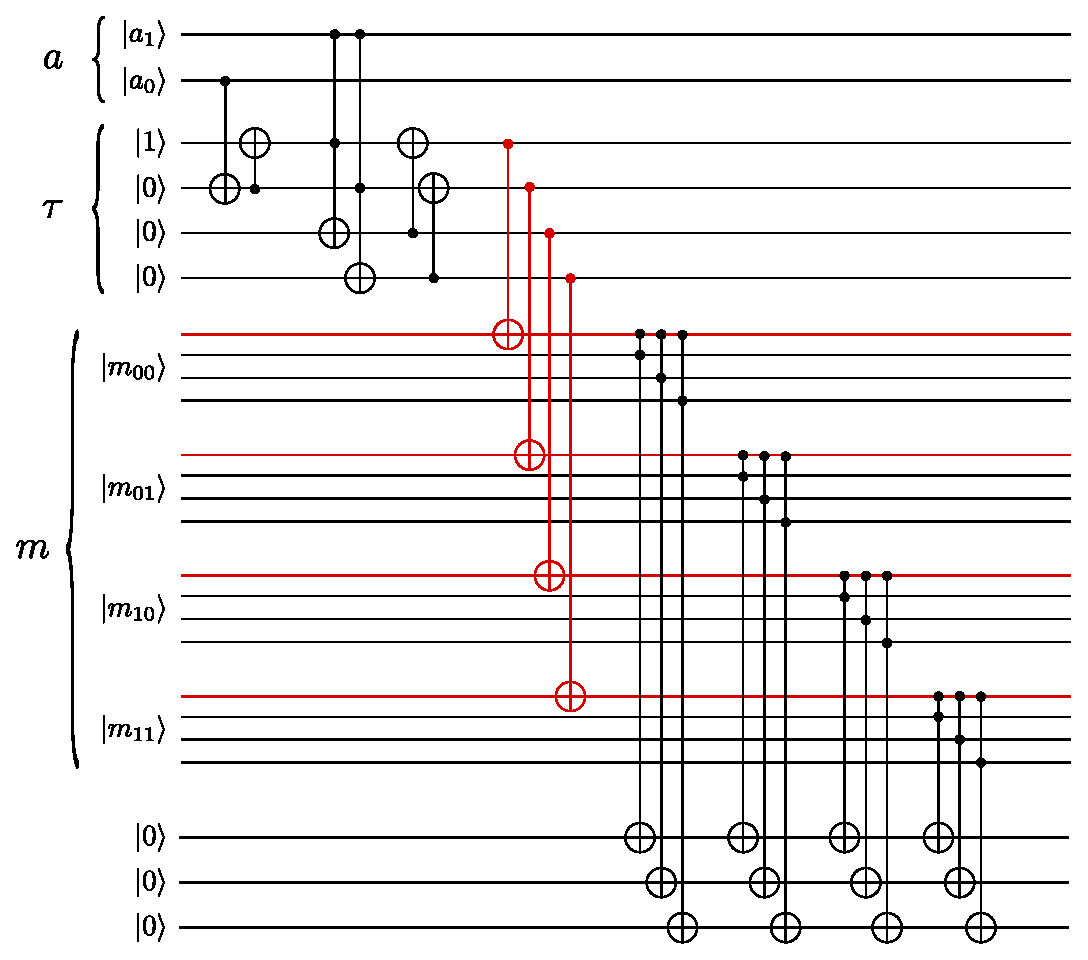
\includegraphics[scale=0.7]{images/bb-2qubit-3bitout}
 \caption{\textbf{For pedagogical purposes; not most optimal.} 
 Extension of the bucket brigade circuit model to the case where each memory cell contains multiple output bits (in this case, 3). 
 The structure of the circuit is largely the same, except now each trigger qubit must perform a Toffoli for every bit in the cell.}
 \label{fig:bb-multioutput}
\end{figure}


\subsubsection{Resource estimation}

One of the primary reasons for designing qRAM libraries in Q\# was to get better resource estimates for qRAM circuits using the functionality afforded to us by both the \texttt{ResourcesEstimator} and the \texttt{ToffoliSimulator}.
Note that all the gates in \autoref{fig:bb-combined} and \autoref{fig:bb-multioutput} are Toffolis, and so bucket brigade qRAMs are really just fancy Boolean circuits. 
Plenty of optimization tools (\textcolor{red}{cite some}) exist for Boolean circuits, and so we anticipate that we'll be able to do reasonably well. 
But first, let's do some resource estimation `by hand' to get an idea of the worst we can expect.

We will do resource estimation at the \emph{logical level}, i.e. not delve into the fault-tolerant level and estimate things like physical qubits and time required. 
Instead, we will focus on the following set of parameters:
\begin{itemize}
 \item Number of qubits $N_q$ (or, circuit width)
 \item Circuit depth $D$
 \item $T$-depth $D_T$
 \item $T$-count $N_T$
 \item CNOT-count $N_{CX}$
 \item non-CNOT Clifford count $N_{HS}$
\end{itemize}
The value of $N_{HS}$ is often not included in lower-level resource estimation. 
For one, on a present-day machine, CNOTs are much noisier and harder to implement, so reducing the number of CNOTs is far more important than reducing the number of other types of gates. 
Furthermore, of the single-qubit gates, the $T$ gate is the one that will give us the most trouble in a fault-tolerant setting. 
The $H$ and $S$ operations are generally considered `easy', but we still include it in our analysis for completeness.

\paragraph{Single-bit output}

Before we begin, we need to make some assumptions. 
All of the gates in a BB circuit are either CNOTs or Toffolis. 
Assuming we choose the typical universal gate of Clifford+$T$, it is necessary to further decompose the Toffolis into elementary gates.
There are a number of ways of doing so, and they differ in that one needs to make a choice about whether to use auxiliary qubits. 
They all require a total of 7 $T$ gates, but the $T$-depth can be decreased with extra qubits. 
There are three `standard' decompositions, and their respective resource counts are shown in \autoref{tab:toffoli-tdepth}. 

In what follows, we will take the simplest route and assume that no auxiliary qubits are added, but note that the resource counts for the $T$-depth 1 case are listed in \cite{DiMatteo2020}. 
We will use the decomposition of Figure 13 in \cite{MITM}, which is reproduced here in \autoref{fig:toffoli-tdepth-3}.

\begin{table}
 \centering
  \captionsetup{width=.89\linewidth}
 \begin{tabular}{|c|c|c|}
  \hline
  Auxiliary qubits & $T$-depth & Reference \\ \hline
  0 & 3 & MITM \\ \hline
  1 & 2 & \todo{Cite} \\ \hline
  3 & 1 & \cite{Selinger2013} \\ \hline
 \end{tabular}
 \caption{A Toffoli gate can be decomposed over Clifford+$T$. 
 While 7 $T$ gates total are required, the $T$-depth is flexible if one chooses to add some additional qubits. \todo{Verify citations} }
 \label{tab:toffoli-tdepth}
\end{table}

\begin{figure}[h]
 \centering
 \captionsetup{width=.89\linewidth}
 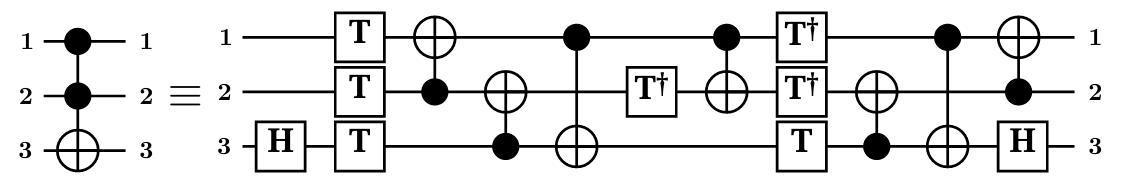
\includegraphics[scale=0.4]{images/matt-toffoli-decomp}
 \caption{A $T$-depth 3 version of the Toffoli gate over Clifford+$T$. 
 This circuit has full depth 9. 
 Figure reproduced from Figure 13 of \cite{MITM}. \todo{remake as vector graphic}}
 \label{fig:toffoli-tdepth-3}
\end{figure}


The number of qubits required was explained previously, but let's total them up. 
Suppose that our memory addresses are $n$ bits. 
Then:
\begin{equation}
 \begin{tabular}{c|c}
  Register & Number  of qubits \\ \hline
  $a$ & $n$ \\
  $\tau$ & $2^n$ \\
  $m$ & $2^n$ \\
  Output & 1 \\ \hline
  Total $N_q$ & $2^{n+1} + n + 1$
 \end{tabular}
\end{equation} 

Next, let's take a closer look at the gate counts. 
In the fanout portion, we see there are $2^n - 2$ Toffolis, and $2^n$ CNOTs. 
In the case where the auxiliary register is being re-used, the fanout portion must be run twice \todo{(depending on how the library handles aux registers, we may not actually need this)}, yielding $2^{n+1} - 4$ Toffolis and $2^{n+1}$ CNOTs. 
As for the query portion, we see there are $2^n$ sequential Toffolis.

Let us begin by computing the $T$-count $N_T$. 
Each Toffoli has 7 $T$-gates, so we have
\begin{eqnarray}
 \nonumber N_T &=& 2 \cdot N_T(\hbox{fanout}) + N_T(\hbox{query}) \\
 \nonumber    &=& 2 \cdot 7 \cdot (2^n - 2) + 7 \cdot 2^n \\
     &=& 21 \cdot 2^n - 28
\end{eqnarray}

Next, the $T$-depth of all the Toffolis. 
Since none of the Toffolis are parallelized, it is just the sum of the $T$-depth of the individual gates:
\begin{eqnarray}
 \nonumber D_T &=& 2 \cdot D_T(\hbox{fanout}) + D_T(\hbox{query}) \\
 \nonumber    &=& 2 \cdot 3 \cdot (2^n - 2) + 3 \cdot 2^n \\
     &=& 9 \cdot 2^n - 12
\end{eqnarray}

The number of non-$CNOT$ Cliffords is also straightforward; only the Toffolis have any such gates: 2 Hadamards per Toffoli. 
Thus,
\begin{eqnarray}
 \nonumber N_{HS} &=& 2 \cdot N_{HS}(\hbox{fanout}) + N_{HS}(\hbox{query}) \\
 \nonumber    &=& 2 \cdot 2 \cdot (2^n - 2) + 2 \cdot 2^n \\
     &=& 6 \cdot 2^n - 8
\end{eqnarray}

For $N_{CX}$, we have
\begin{eqnarray}
 \nonumber N_{CX} &=& 2 \cdot N_{CX}(\hbox{fanout}) + N_{CX}(\hbox{query}) \\
 \nonumber    &=& 2 \cdot \left(7 \cdot (2^n - 2) + 2^n \right)  + 7 \cdot 2^n \\
     &=& 23 \cdot 2^n - 28
\end{eqnarray}

Finally, let's compute the depth. 
Note that in the fanout portion, the CNOTs can be run in only $n + 1$ layers of depth because many of the cascades can be parallelized. 
The depth of the Toffolis, however, is fixed at 9, so we obtain:
\begin{eqnarray}
 \nonumber D &=& 2 \cdot D (\hbox{fanout}) + D (\hbox{query}) \\
 \nonumber    &=& 2 \cdot \left(9 \cdot (2^n - 2) +n + 1 \right) + 9 \cdot 2^n \\
     &=& 27 \cdot 2^n + 2n -34
\end{eqnarray}

The final (unoptimized) resource counts for a one-bit bucket brigade qRAM are:
\begin{eqnarray}
 N_q &=& 2^{n+1} + n + 1 \\ \nonumber
 D   &=& 27 \cdot 2^n + 2n -34 \\ \nonumber
 D_T &=& 9 \cdot 2^n - 12 \\ \nonumber
 N_T &=& 21 \cdot 2^n - 28 \\ \nonumber
 N_{CX} &=& 23 \cdot 2^n - 28 \\ \nonumber
 N_{HS} &=& 6 \cdot 2^n - 8
\end{eqnarray}
 
 
 \todo{VERIFY and cross-check with \texttt{ResourcesEstimator} and our library code.}
 
\paragraph{Multi-bit output}

Let us now perform the same analysis for the situation where the memory cells may store multiple bits.
We'll suppose that addresses are still $n$ bits, but store $k$ bits each. 
Consider the differences between the top right panel of \autoref{fig:bb-combined}, and \autoref{fig:bb-multioutput} (i.e. a 2-bit address, so 4 memory cells). 
The address fanout portion is \emph{exactly the same}; what differs is the query itself, as now we need to couple with each of the memory cells to copy the information to the output.
The number of qubits of course increases:
\begin{equation}
 \begin{tabular}{c|c}
  Register & Number  of qubits \\ \hline
  $a$ & $n$ \\
  $\tau$ & $2^n$ \\
  $m$ & $k \cdot 2^n$ \\
  Output & $k$ \\ \hline
  Total $N_q$ & $(k + 1) 2^n + n + k$
 \end{tabular}
\end{equation} 
Then each of the $2^n$ Toffolis of the query portion is replaced with $k$ Toffolis, one per output bit.
Note, however, that many of these Toffolis can in fact be done in parallel. 
We will not consider that when estimating resources here by hand, but note that once we implement the circuits in Q\# and use the Toffoli simulator, the circuit depth will likely decrease significantly.
Calculating by hand, the resources for the multi-output bit case are as follows:
\begin{eqnarray}
 N_q &=& (k + 1) 2^n + n + k \\ \nonumber
 D   &=& (18 + 9k)2^n + 2n - 34 \\ \nonumber
 D_T &=& (6+3k)2^n - 12 \\ \nonumber
 N_T &=& (14 + 7k)2^n - 28 \\ \nonumber
 N_{CX} &=& (16+7k)2^n - 28  \\ \nonumber
 N_{HS} &=& (4+2k)2^n - 8
\end{eqnarray}

\todo{Verify and cross-check with \texttt{ResourcesEstimator}}

\subsection{Phase query circuit model}

\subsubsection{Resource estimation}


%%%%%%%%%%%%%%%%%%%%%%%%%%%%%%%%%%%%%%%%%%%%%%%%%%%%%%%%%%%%%%%%%%%%%%%%%%%%%%%%%%
%%%%%%%%%%%%%%%%%%%%%%%%%%%%%%%%%%%%%%%%%%%%%%%%%%%%%%%%%%%%%%%%%%%%%%%%%%%%%%%%%%
%%%%%%%%%%%%%%%%%%%%%%%%%%%%%%%%%%%%%%%%%%%%%%%%%%%%%%%%%%%%%%%%%%%%%%%%%%%%%%%%%%
%%%%%%%%%%%%%%%%%%%%%%%%%%%%%%%%%%%%%%%%%%%%%%%%%%%%%%%%%%%%%%%%%%%%%%%%%%%%%%%%%%
%%%%%%%%%%%%%%%%%%%%%%%%%%%%%%%%%%%%%%%%%%%%%%%%%%%%%%%%%%%%%%%%%%%%%%%%%%%%%%%%%%

\section{Quantum ROM}
\label{sec:circuits}

\subsection{Quantum ROM}

\subsection{Efficient state preparation with a qROM}

Discuss \cite{Vadym2018}

\subsection{Optimizing quantum ROMs}

\subsection{Problem-specific qROMs}

Talk about the qROM in \cite{Babbush2018}
%%%%%%%%%%%%%%%%%%%%%%%%%%%%%%%%%%%%%%%%%%%%%%%%%%%%%%%%%%%%%%%%%%%%%%%%%%%%%%%%%%
%%%%%%%%%%%%%%%%%%%%%%%%%%%%%%%%%%%%%%%%%%%%%%%%%%%%%%%%%%%%%%%%%%%%%%%%%%%%%%%%%%
%%%%%%%%%%%%%%%%%%%%%%%%%%%%%%%%%%%%%%%%%%%%%%%%%%%%%%%%%%%%%%%%%%%%%%%%%%%%%%%%%%
%%%%%%%%%%%%%%%%%%%%%%%%%%%%%%%%%%%%%%%%%%%%%%%%%%%%%%%%%%%%%%%%%%%%%%%%%%%%%%%%%%
%%%%%%%%%%%%%%%%%%%%%%%%%%%%%%%%%%%%%%%%%%%%%%%%%%%%%%%%%%%%%%%%%%%%%%%%%%%%%%%%%%

\section{Hardware proposals for qRAM}
\label{sec:hardware}



%%%%%%%%%%%%%%%%%%%%%%%%%%%%%%%%%%%%%%%%%%%%%%%%%%%%%%%%%%%%%%%%%%%%%%%%%%%%%%%%%%
%%%%%%%%%%%%%%%%%%%%%%%%%%%%%%%%%%%%%%%%%%%%%%%%%%%%%%%%%%%%%%%%%%%%%%%%%%%%%%%%%%
%%%%%%%%%%%%%%%%%%%%%%%%%%%%%%%%%%%%%%%%%%%%%%%%%%%%%%%%%%%%%%%%%%%%%%%%%%%%%%%%%%
%%%%%%%%%%%%%%%%%%%%%%%%%%%%%%%%%%%%%%%%%%%%%%%%%%%%%%%%%%%%%%%%%%%%%%%%%%%%%%%%%%
%%%%%%%%%%%%%%%%%%%%%%%%%%%%%%%%%%%%%%%%%%%%%%%%%%%%%%%%%%%%%%%%%%%%%%%%%%%%%%%%%%

\section{Outlook}
\label{sec:outlook}

%%%%%%%%%%%%%%%%%%%%%%%%%%%%%%%%%%%%%%%%%%%%%%%%%%%%%%%%%%%%%%%%%%%%%%%%%%%%%%%%%%
%%%%%%%%%%%%%%%%%%%%%%%%%%%%%%%%%%%%%%%%%%%%%%%%%%%%%%%%%%%%%%%%%%%%%%%%%%%%%%%%%%
%%%%%%%%%%%%%%%%%%%%%%%%%%%%%%%%%%%%%%%%%%%%%%%%%%%%%%%%%%%%%%%%%%%%%%%%%%%%%%%%%%
%%%%%%%%%%%%%%%%%%%%%%%%%%%%%%%%%%%%%%%%%%%%%%%%%%%%%%%%%%%%%%%%%%%%%%%%%%%%%%%%%%
%%%%%%%%%%%%%%%%%%%%%%%%%%%%%%%%%%%%%%%%%%%%%%%%%%%%%%%%%%%%%%%%%%%%%%%%%%%%%%%%%%

\bibliography{primer}
\bibliographystyle{unsrt}

\end{document}
